\documentclass[11pt,a4paper,english,twoside]{article}

\usepackage{a4wide}
\usepackage{amssymb,amsmath,amsthm}
\usepackage{graphicx}
\usepackage{subcaption}
\usepackage[pdftex,hyperref,svgnames]{xcolor}
\usepackage[pdftex,colorlinks=true,
pdfstartview=FitV,
pdfnewwindow=true,
linktoc=page,
linkcolor=blue,
citecolor=red,
urlcolor=blue,
hyperindex=true,
hyperfigures=false]{hyperref}
\hypersetup{linktocpage}
\usepackage{dsfont}
\usepackage{empheq}
\usepackage{float}
\usepackage{enumerate}
\usepackage{enumitem}
\usepackage{setspace}
\usepackage{xcolor}
\usepackage{listings}

\graphicspath{{doc/figures/}{figures/}}

% --- code listing styles for the before/after section ---
\definecolor{codebg}{rgb}{0.97,0.97,0.97}
\definecolor{codekw}{rgb}{0.10,0.10,0.60}
\definecolor{codecmt}{rgb}{0.30,0.50,0.30}
\lstdefinestyle{cstyle}{
  language=C,
  basicstyle=\ttfamily\scriptsize,
  keywordstyle=\color{codekw},
  commentstyle=\color{codecmt},
  backgroundcolor=\color{codebg},
  breaklines=true,
  columns=fullflexible,
  showstringspaces=false,
  frame=single,
  framesep=3pt,
  xleftmargin=4pt,
  literate={->}{{->}}2
}
\newcommand{\codefile}[1]{\smallskip\noindent\texttt{\small #1}\par\nopagebreak}

\newcommand{\nn}{\nonumber}
\def\beq{\begin{equation}}
\def\eeq{\end{equation}}
\def\bea{\begin{eqnarray}}
\def\eea{\end{eqnarray}}
\def\del{\partial}
\def\d{{\rm d}}
\def\cH{{\cal H}}
\def\Am{A_m}
\def\Ar{A_r}
\def\rhob{\bar\rho}
\def\rhode{\rho_{\rm DE}}
\def\wde{w_{\rm DE}}

\begin{document}
\numberwithin{equation}{section}

\begin{center}
{\Large \bf CLASS implementation note: scalar-field couplings to matter and dark radiation}\\[5pt]
{\normalsize Branch \texttt{DE\_DR\_DM\_int}}
\end{center}

\section{Purpose and conventions}

This note summarizes the CLASS implementation of scalar-field couplings to matter and
dark radiation, following the conventions of
\path{REFS_FOR_CLAUDE/NotesRadiationCoupling260616.tex}.  The paper example for
the matter-coupled model is \path{2505.10410v2.pdf}; the two radiation-coupled
models are those of \path{NotesRadiationCoupling_DONTTOUCH.pdf}.

We use a scalar field $\phi$ with potential $V(\phi)$ and multiplicative coupling
functions $\Am(\phi)$ and $\Ar(\phi)$ such that
\beq
\rho_m = \Am(\phi)\,\rhob_m,\qquad
\rho_r = \Ar(\phi)\,\rhob_r,\qquad
\rhob_m\propto a^{-3},\qquad \rhob_r\propto a^{-4}.
\label{eq:bgdensities}
\eeq
The fiducial background values used in the comparison runs are
\bea
\Omega_{r0}=10^{-4},\qquad
\Omega_{m0}=0.3149,\qquad
\Omega_{\phi0}=0.6850,\qquad
\Omega_{k0}=0.
\eea

All implementation changes are inside CLASS.  The external scripts used during
development only read CLASS output tables and produced the figures included below.

\section{Matter-coupled scalar background}

For the matter sector, the new form is
\beq
\Am(\phi)=1+C_m\left(1-e^{-\beta_m\phi}\right),\qquad
C(\phi)=\Am(\phi)^2.
\label{eq:amform}
\eeq
In the code this is selected by
\beq
\texttt{scf\_conformal\_form = matter\_exp}.
\eeq
The existing qcdm--scalar conformal machinery is then reused through
\texttt{C\_scf}, \texttt{dC\_scf}, \texttt{ddC\_scf}, \texttt{Q\_scf}, and the
existing perturbed \texttt{delta\_Q\_scf} coefficients.

The option
\beq
\texttt{scf\_ic\_from\_today = yes}
\eeq
reconstructs $\phi_{\rm ini}$, $\phi'_{\rm ini}$, $V_0$, and the initial qcdm
density from the requested today values.  This is used by
\texttt{fig3\_2505\_matter.ini}.  The slope used for the Fig.~3 reproduction is
\beq
\lambda=\sqrt{2},
\eeq
as in Eq.~(3.8) of \texttt{2505.10410v2.pdf}.

For this case the effective dark-energy variables are
\beq
\rhode=\rho_\phi+(\Am-1)\rhob_m,\qquad
\wde\,\rhode=p_\phi.
\label{eq:deeffmatter}
\eeq

\begin{figure}[H]
\centering
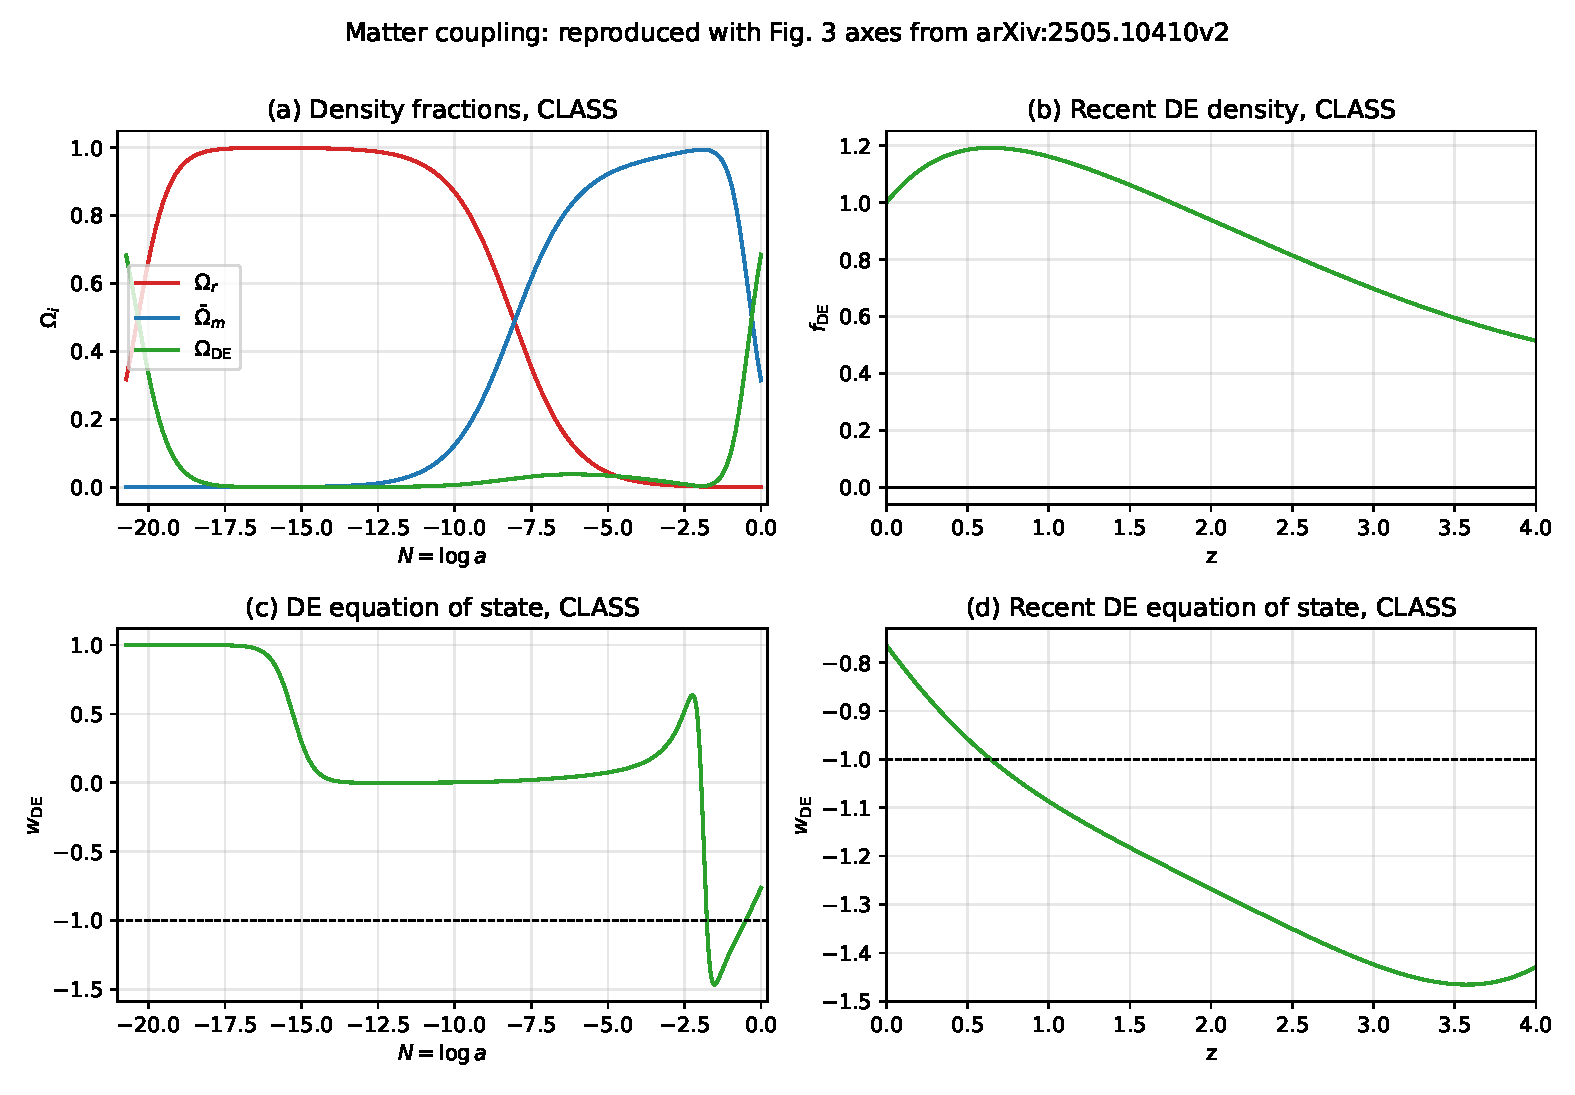
\includegraphics[width=0.95\textwidth]{matter_coupling_fig3_comparison.pdf}
\caption{Matter-coupled CLASS reproduction for the \texttt{fig3\_2505\_matter.ini}
setup.  The plotted matter fraction uses $\rhob_m=\rho_{\rm qcdm}/\Am$.}
\label{fig:matter}
\end{figure}

At $z=0$, the CLASS output gives
\begin{center}
\begin{tabular}{c|c}
quantity & CLASS value\\
\hline
$w_{\phi0}$ & $-0.763660007$\\
$w_{{\rm DE}0}$ & $-0.763660007$\\
$\Omega_{r0}$ & $9.9999997\times10^{-5}$\\
$\Omega_{m0}$ & $0.314900009$\\
$\Omega_{{\rm DE}0}$ & $0.684999991$\\
$\phi_0$ & $-1.31\times10^{-8}$
\end{tabular}
\end{center}

\section{Radiation-coupled scalar background}

The radiation coupling is independent of the qcdm conformal factor.  It is selected by
\beq
\texttt{scf\_interacting\_radiation = yes}
\eeq
and uses the free parameters \texttt{scf\_C0\_r} and \texttt{scf\_beta\_r}:
\beq
\Ar(\phi)=1+C_r\left(1-e^{-\beta_r\phi}\right).
\label{eq:arform}
\eeq
The CLASS background density stored in \texttt{rho\_idr} is the full coupled density,
\beq
\rho_{\rm idr}=\Ar(\phi)\,\rhob_{\rm idr}.
\label{eq:rhoidr}
\eeq
The pressure is kept as radiation,
\beq
p_{\rm idr}=\frac13\rho_{\rm idr}.
\eeq

The normalization of the radiation Lagrangian only fixes the field amplitude inside
$\rhob_{\rm idr}$.  The implemented object is the radiation stress tensor,
\beq
T^0{}_0=-\rho_{\rm idr},\qquad
T^i{}_j=\frac13\rho_{\rm idr}\delta^i_j,
\label{eq:radtensor}
\eeq
so $\Ar$ rescales the full dark-radiation tensor.  The anisotropic-stress hierarchy
is otherwise the existing CLASS idr hierarchy.

The scalar background equation is implemented in CLASS density units as
\beq
\phi''+2\cH\phi'+a^2\left(V_{,\phi}-Q_m-Q_r\right)=0,\qquad
Q_r=-3\rho_{\rm idr}\,\frac{\del_\phi\Ar}{\Ar}.
\label{eq:bgkgclass}
\eeq
This sign matches the physical equation
\beq
\ddot\phi+3H\dot\phi+V_{,\phi}+\rhob_m\del_\phi\Am+\rhob_r\del_\phi\Ar=0,
\label{eq:bgkgphysical}
\eeq
after using the CLASS convention in which densities are multiplied by
$8\pi G/3$.

The effective dark-energy output is
\beq
\rhode=\rho_\phi+(\Am-1)\rhob_m+(\Ar-1)\rhob_r,
\label{eq:deeffrho}
\eeq
\beq
\wde\,\rhode=p_\phi+\frac13(\Ar-1)\rhob_r.
\label{eq:deeffw}
\eeq

\begin{figure}[H]
\centering
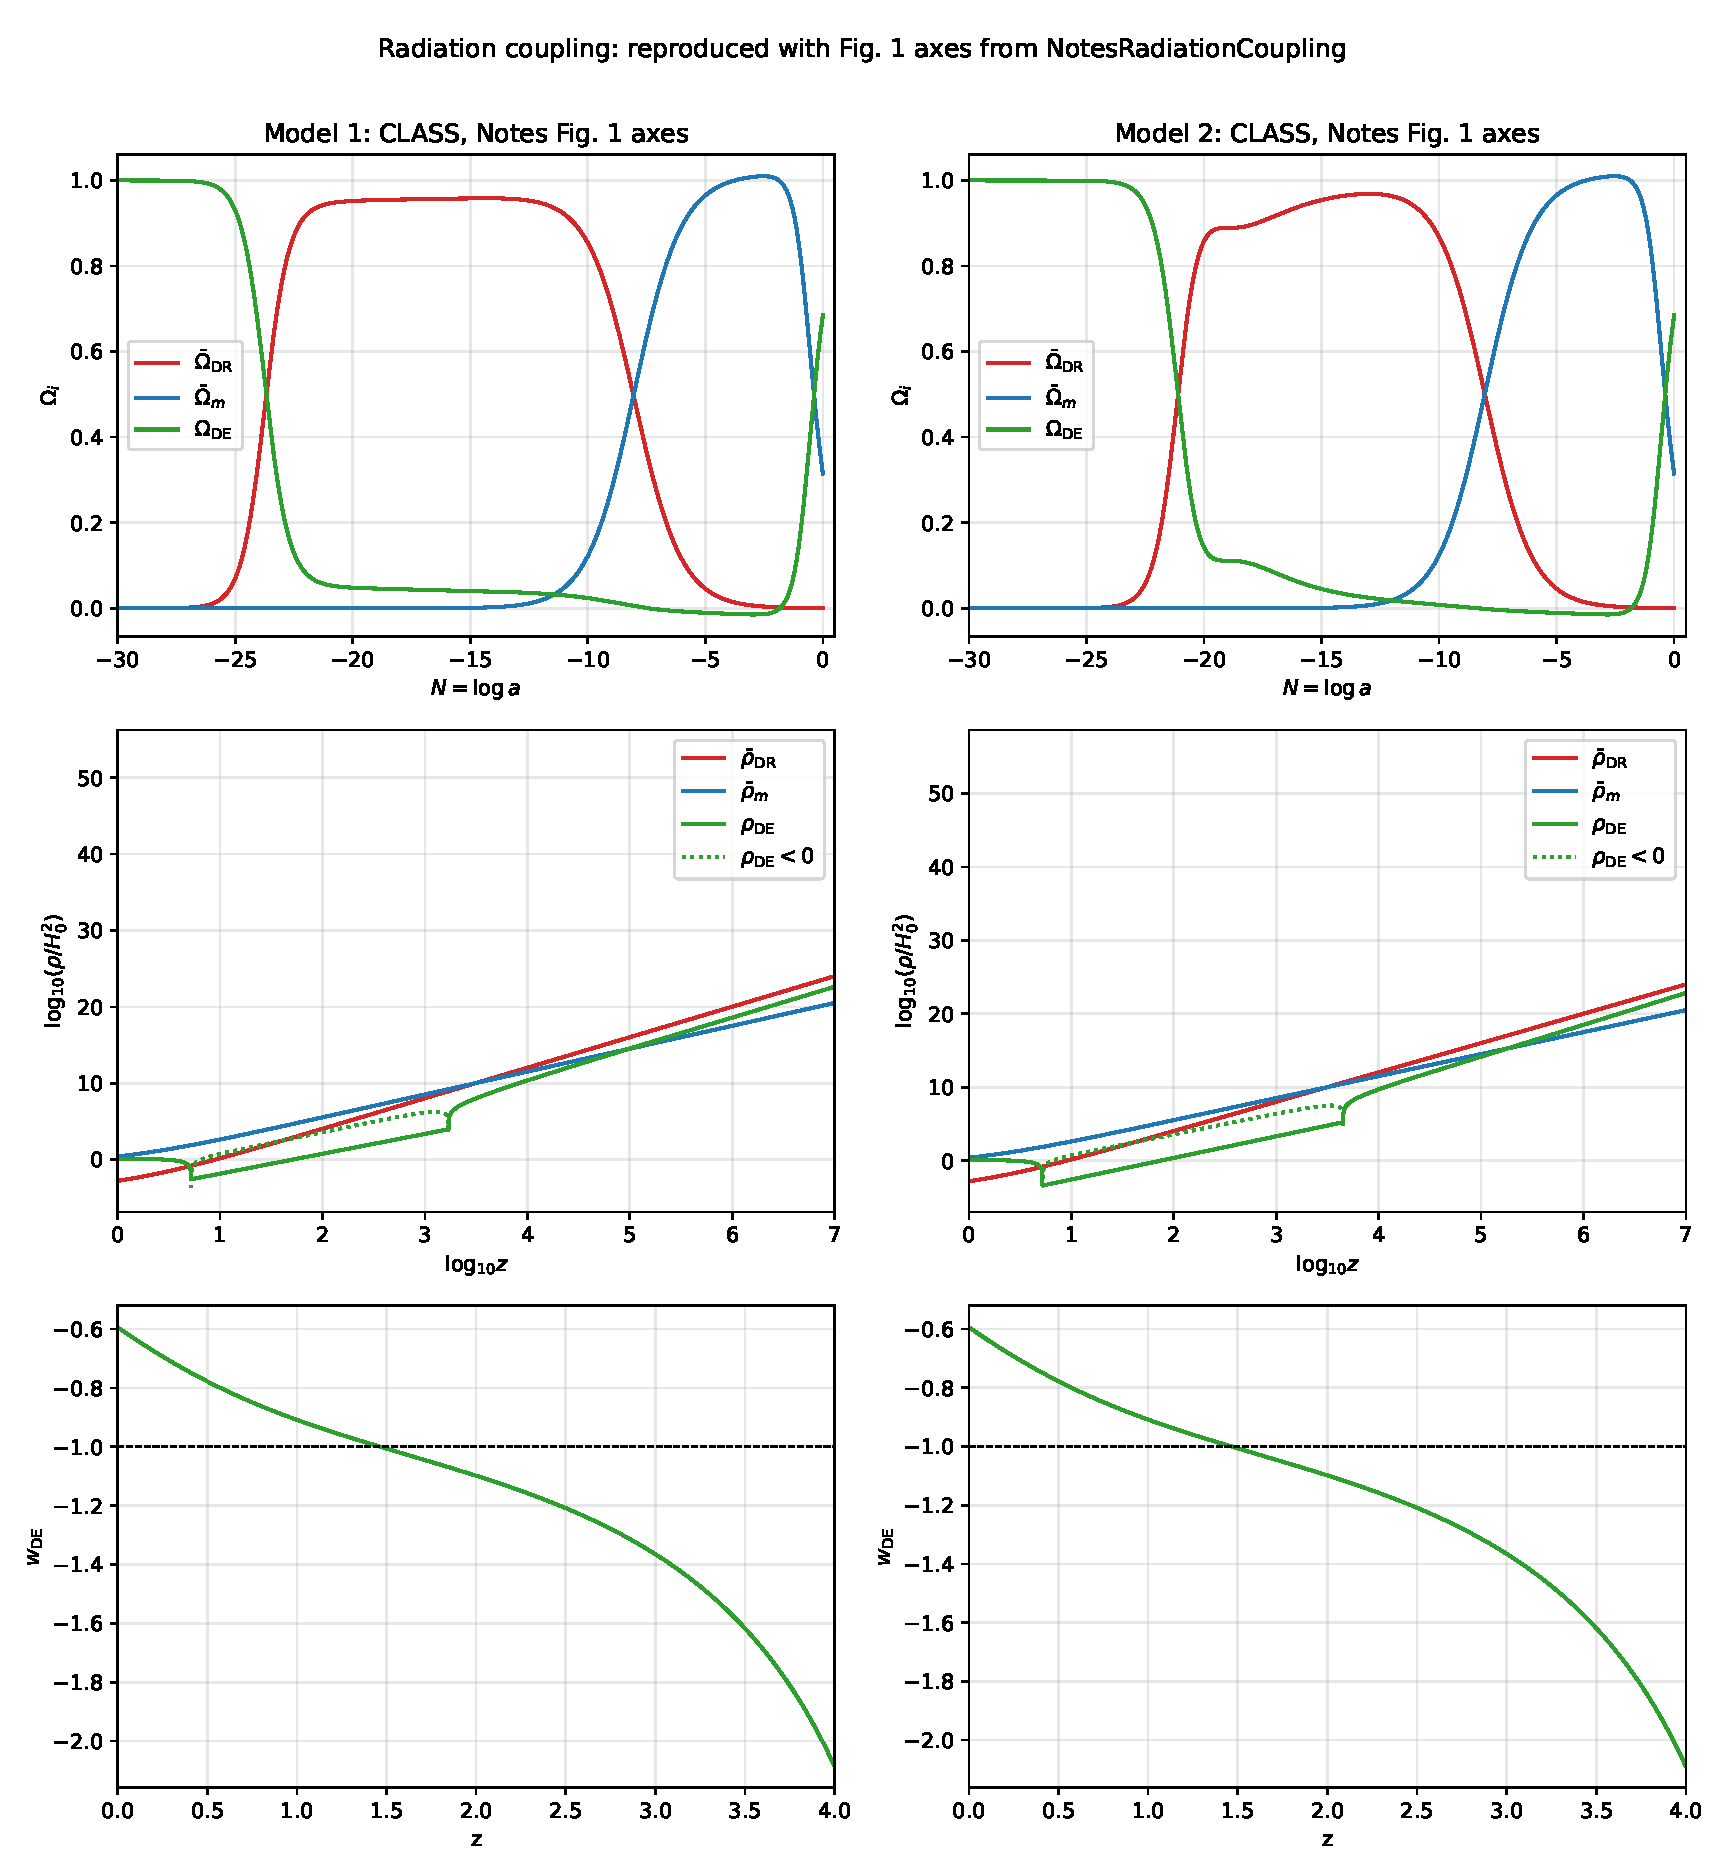
\includegraphics[width=0.98\textwidth]{radiation_coupling_fig1_comparison.pdf}
\caption{Radiation-coupled CLASS reproduction for the two
\texttt{NotesRadiationCoupling} Fig.~1 models.  The plotted barred radiation and
matter densities are reconstructed as
$\rhob_r=\rho_{\rm idr}/\Ar$ and $\rhob_m=\rho_{\rm qcdm}/\Am$.}
\label{fig:radiation}
\end{figure}

At $z=0$, the two Notes models give
\begin{center}
\begin{tabular}{c|cc}
quantity & model 1 & model 2\\
\hline
$w_{\phi0}$ & $-0.594208876$ & $-0.594223632$\\
$w_{{\rm DE}0}$ & $-0.594208863$ & $-0.594223633$\\
$\Omega_{r0}$ & $1.0000022\times10^{-4}$ & $9.9999990\times10^{-5}$\\
$\Omega_{m0}$ & $0.314899728$ & $0.314900018$\\
$\Omega_{{\rm DE}0}$ & $0.685000288$ & $0.684999981$\\
$\phi_0$ & $1.30\times10^{-6}$ & $-5.69\times10^{-8}$\\
$\Ar(\phi_0)$ & $0.999999901$ & $1.000000001$
\end{tabular}
\end{center}

\section{Radiation perturbations}

The perturbations are implemented for the full coupled idr variables
\beq
\delta_{\rm idr}\equiv\frac{\delta\rho_{\rm idr}}{\rho_{\rm idr}},\qquad
\theta_{\rm idr}.
\eeq
Define
\beq
\Lambda_r\equiv\frac{\del_\phi\Ar}{\Ar},\qquad
\Lambda_{2,r}\equiv\frac{\d^2\ln\Ar}{\d\phi^2}
=\frac{\del^2_\phi\Ar}{\Ar}-\Lambda_r^2.
\label{eq:lambdar}
\eeq
In synchronous gauge, the added idr terms are
\beq
\delta_{\rm idr}' =
-\frac43\left(\theta_{\rm idr}+\frac{h'}{2}\right)
+\Lambda_r\,\delta\phi'
+\Lambda_{2,r}\,\phi'\,\delta\phi,
\label{eq:deltaidr}
\eeq
\beq
\theta_{\rm idr}' =
\frac{k^2}{4}\delta_{\rm idr}
-k^2\sigma_{\rm idr}
+\frac34\Lambda_r k^2\delta\phi
-\Lambda_r\phi'\theta_{\rm idr}.
\label{eq:thetaidr}
\eeq
IDM--DR scattering terms, when present, are preserved and the scalar force is added
on top of the usual idr Euler equation.

The scalar perturbation equation receives
\beq
\delta Q_r=-3\rho_{\rm idr}
\left(\Lambda_r\delta_{\rm idr}+\Lambda_{2,r}\delta\phi\right),
\label{eq:deltaqr}
\eeq
which enters the perturbed Klein--Gordon equation as $a^2\delta Q_r$, analogously to
the existing qcdm \texttt{delta\_Q\_scf} term.  In Newtonian gauge the metric term
$2\psi Q_r$ is added in the same way as for the qcdm source.

\section{Code changes: before and after}
\label{sec:beforeafter}

This section documents the concrete code edits behind the equations above, as
\emph{before}/\emph{after} pairs taken from the three implementation commits
(\texttt{11432659}, \texttt{2f4abc0d}, \texttt{dfb1975c}) relative to the
pre-implementation state (\texttt{74a2ed72}).  Line numbers refer to the current
tree.  Blocks marked ``new'' had no prior counterpart.

\subsection{\texttt{source/background.c}: matter conformal form}

The conformal factor selector gained the \texttt{matter\_exp} branch
$C(\phi)=A_m(\phi)^2$ with $A_m=1+C_m(1-e^{-\beta_m\phi})$
[Eq.~\eqref{eq:amform}].  Shown for \texttt{C\_scf}; \texttt{dC\_scf} and
\texttt{ddC\_scf} were extended identically.

\codefile{Before (\texttt{C\_scf}, only the exponential form existed):}
\begin{lstlisting}[style=cstyle]
switch (pba->scf_conformal_form) {
  case scf_conformal_exp:
    return scf_C0*exp(2.*scf_beta*phi);
  default:
    class_stop(pba->error_message, "Unknown scf_conformal_form %d", pba->scf_conformal_form);
    return 1.0;
}
\end{lstlisting}

\codefile{After (new \texttt{matter\_exp} case, plus a shared helper):}
\begin{lstlisting}[style=cstyle]
static void scf_matter_exp_A(struct background *pba, double phi,
                             double *A, double *dA, double *ddA) {
  double Aphi = pba->C0_scf, alpha = pba->beta_scf, e = exp(-alpha*phi);
  *A   = 1.0 + Aphi*(1.0 - e);
  *dA  = Aphi*alpha*e;
  *ddA = -Aphi*alpha*alpha*e;
}
/* ... inside C_scf: */
switch (pba->scf_conformal_form) {
  case scf_conformal_exp:
    return scf_C0*exp(2.*scf_beta*phi);
  case scf_conformal_matter_exp:          /* NEW */
    scf_matter_exp_A(pba,phi,&A,&dA,&ddA);
    return A*A;
  default:
    class_stop(pba->error_message, "Unknown scf_conformal_form %d", pba->scf_conformal_form);
    return 1.0;
}
\end{lstlisting}

\subsection{\texttt{source/background.c}: radiation coupling function (new)}

The multiplicative radiation factor $A_r$ and its derivatives
[Eq.~\eqref{eq:arform}] were added with the same exponential template:

\codefile{New (\texttt{source/background.c}, $\sim$l.\,3661--3715):}
\begin{lstlisting}[style=cstyle]
static void scf_radiation_exp_A(struct background *pba, double phi,
                                double *A, double *dA, double *ddA) {
  double Aphi = pba->C0_r_scf, beta = pba->beta_r_scf, e = exp(-beta*phi);
  *A   = 1.0 + Aphi*(1.0 - e);
  *dA  = Aphi*beta*e;
  *ddA = -Aphi*beta*beta*e;
}
double  A_r_scf(...) { ... return A;  }   /* A_r(phi)        */
double dA_r_scf(...) { ... return dA; }   /* d A_r / dphi    */
double ddA_r_scf(...){ ... return ddA;}   /* d^2 A_r / dphi^2 */
\end{lstlisting}

\subsection{\texttt{source/background.c}: coupled \texttt{rho\_idr}}

The interacting-dark-radiation density is multiplied by $A_r(\phi)$ so that
\texttt{rho\_idr} stores the full coupled density [Eq.~\eqref{eq:rhoidr}].

\codefile{Before ($\sim$l.\,630):}
\begin{lstlisting}[style=cstyle]
if (pba->has_idr == _TRUE_) {
  pvecback[pba->index_bg_rho_idr] = pba->Omega0_idr * pow(pba->H0,2) / pow(a,4);
  rho_tot += pvecback[pba->index_bg_rho_idr];
  ...
}
\end{lstlisting}
\codefile{After:}
\begin{lstlisting}[style=cstyle]
if (pba->has_idr == _TRUE_) {
  pvecback[pba->index_bg_rho_idr] = pba->Omega0_idr * pow(pba->H0,2) / pow(a,4);
  if (pba->has_scf_radiation == _TRUE_) {                 /* NEW */
    pvecback[pba->index_bg_rho_idr] *= A_r_scf(pba,phi);   /* NEW */
  }
  rho_tot += pvecback[pba->index_bg_rho_idr];
  ...
}
\end{lstlisting}

\subsection{\texttt{source/background.c}: scalar background equation}

The background Klein--Gordon source $-Q$ in $\phi''+2\cH\phi'+a^2(V_{,\phi}-Q)=0$
gained the radiation term $Q_r=-3\rho_{\rm idr}\,\del_\phi A_r/A_r$
[Eq.~\eqref{eq:bgkgclass}].

\codefile{Before ($\sim$l.\,3105):}
\begin{lstlisting}[style=cstyle]
if (pba->has_scf == _TRUE_) {
  double Q_bg_scf = 0.;
  if (pba->has_qcdm_de_q == _TRUE_) {
    Q_bg_scf = Q_scf(pba, y[..phi], y[..phi_prime], y[..rho_qcdm], a, pvecback);
  }
  dy[pba->index_bi_phi_scf] = y[pba->index_bi_phi_prime_scf]/a/H;
  ...
}
\end{lstlisting}
\codefile{After:}
\begin{lstlisting}[style=cstyle]
if (pba->has_scf == _TRUE_) {
  double Q_bg_scf = 0.;
  if (pba->has_qcdm_de_q == _TRUE_) {
    Q_bg_scf = Q_scf(pba, y[..phi], y[..phi_prime], y[..rho_qcdm], a, pvecback);
  }
  if (pba->has_scf_radiation == _TRUE_) {                      /* NEW */
    double A_r = A_r_scf(pba, y[pba->index_bi_phi_scf]);
    class_test(A_r <= 0., error_message, "A_r(phi) = %e must stay positive.", A_r);
    /* rho_idr stores A_r rho_bar_r; CLASS units give Q_r = -3 rho_bar_r A_r,phi */
    Q_bg_scf += -3.0*(pvecback[pba->index_bg_rho_idr]/A_r)*dA_r_scf(pba, y[pba->index_bi_phi_scf]);
  }
  dy[pba->index_bi_phi_scf] = y[pba->index_bi_phi_prime_scf]/a/H;
  ...
}
\end{lstlisting}

\subsection{\texttt{source/background.c}: effective dark-energy output (new)}

The output block was extended to print $\rho_{\rm DE}$ and $w_{\rm DE}$ including
the radiation term [Eqs.~\eqref{eq:deeffrho}--\eqref{eq:deeffw}]:

\codefile{New ($\sim$l.\,2924):}
\begin{lstlisting}[style=cstyle]
double A_r       = (pba->has_scf_radiation==_TRUE_) ? pvecback[pba->index_bg_A_r_scf] : 1.0;
double rho_bar_r = (pba->has_scf_radiation==_TRUE_) ? pvecback[pba->index_bg_rho_idr]/A_r : 0.0;
double matter_coupling = 0.0;
if (pba->has_qcdm_de_q == _TRUE_) {
  double A_scf = sqrt(pvecback[pba->index_bg_C_scf]);          /* A_m = sqrt(C) */
  matter_coupling = pvecback[pba->index_bg_rho_qcdm]*(1.0 - 1.0/A_scf);
}
double rho_de_eff = pvecback[pba->index_bg_rho_scf] + matter_coupling + (A_r-1.0)*rho_bar_r;
double p_de_eff   = pvecback[pba->index_bg_p_scf]   + (1.0/3.0)*(A_r-1.0)*rho_bar_r;
\end{lstlisting}

\subsection{\texttt{source/perturbations.c}: coupling coefficients (new)}

$\Lambda_r$, $\Lambda_{2,r}$ and $Q_r$ [Eq.~\eqref{eq:lambdar}] are precomputed
once per call:

\codefile{New ($\sim$l.\,9365):}
\begin{lstlisting}[style=cstyle]
if (use_radiation == _TRUE_) {
  lambda_r_scf  = pvecback[pba->index_bg_dA_r_scf]/pvecback[pba->index_bg_A_r_scf];
  lambda2_r_scf = pvecback[pba->index_bg_ddA_r_scf]/pvecback[pba->index_bg_A_r_scf]
                  - lambda_r_scf*lambda_r_scf;
  Q_r_scf       = -3.0*pvecback[pba->index_bg_rho_idr]*lambda_r_scf;
}
\end{lstlisting}

\subsection{\texttt{source/perturbations.c}: idr continuity and Euler}

The two source terms of Eqs.~\eqref{eq:deltaidr}--\eqref{eq:thetaidr} are added on
top of the standard idr fluid equations.

\codefile{Before ($\sim$l.\,9979):}
\begin{lstlisting}[style=cstyle]
dy[pv->index_pt_delta_idr] = -4./3.*(theta_idr + metric_continuity);
...
dy[pv->index_pt_theta_idr] = k2*(y[pv->index_pt_delta_idr]/4.-s2_squared*y[pv->index_pt_shear_idr]) + metric_euler;
\end{lstlisting}
\codefile{After:}
\begin{lstlisting}[style=cstyle]
dy[pv->index_pt_delta_idr] = -4./3.*(theta_idr + metric_continuity);
if (use_radiation == _TRUE_) {                                       /* NEW */
  dy[pv->index_pt_delta_idr] +=
      lambda_r_scf*y[pv->index_pt_phi_prime_scf]
    + lambda2_r_scf*pvecback[pba->index_bg_phi_prime_scf]*y[pv->index_pt_phi_scf];
}
...
dy[pv->index_pt_theta_idr] = k2*(y[pv->index_pt_delta_idr]/4.-s2_squared*y[pv->index_pt_shear_idr]) + metric_euler;
if (use_radiation == _TRUE_) {                                       /* NEW */
  dy[pv->index_pt_theta_idr] +=
      0.75*lambda_r_scf*k2*y[pv->index_pt_phi_scf]
    - lambda_r_scf*pvecback[pba->index_bg_phi_prime_scf]*theta_idr;
}
\end{lstlisting}

\subsection{\texttt{source/perturbations.c}: perturbed Klein--Gordon source}

The radiation source $\delta Q_r$ [Eq.~\eqref{eq:deltaqr}] is built and injected
into the perturbed KG equation as $a^2\delta Q_r$, with the Newtonian-gauge
$2\psi Q_r$ term, mirroring the qcdm \texttt{delta\_Q\_scf} source.

\codefile{Before (synchronous KG, no radiation term):}
\begin{lstlisting}[style=cstyle]
dy[pv->index_pt_phi_prime_scf] =
    -2.*a_prime_over_a*y[pv->index_pt_phi_prime_scf]
    -(k2+a2*pvecback[pba->index_bg_ddV_scf])*y[pv->index_pt_phi_scf]
    -metric_continuity*pvecback[pba->index_bg_phi_prime_scf]
    + kg_term_entropy + kg_term_q;
\end{lstlisting}
\codefile{After (source assembled, then added):}
\begin{lstlisting}[style=cstyle]
if (use_radiation == _TRUE_) {                                       /* NEW */
  delta_Q_r_scf = Q_r_scf*delta_idr
                - 3.0*pvecback[pba->index_bg_rho_idr]*lambda2_r_scf*y[pv->index_pt_phi_scf];
}
...
double kg_term_r = 0.;
if (use_radiation == _TRUE_) {                                       /* NEW */
  kg_term_r = a2*delta_Q_r_scf;
  if (ppt->gauge == newtonian)
    kg_term_r += 2.*a2*pvecmetric[ppw->index_mt_psi]*Q_r_scf;
}
dy[pv->index_pt_phi_prime_scf] =
    -2.*a_prime_over_a*y[pv->index_pt_phi_prime_scf]
    -(k2+a2*pvecback[pba->index_bg_ddV_scf])*y[pv->index_pt_phi_scf]
    -metric_continuity*pvecback[pba->index_bg_phi_prime_scf]
    + kg_term_entropy + kg_term_q + kg_term_r;                       /* + kg_term_r NEW */
\end{lstlisting}

\subsection{\texttt{source/input.c} and \texttt{include/background.h}}

Parsing of the new switches and storage of the new parameters/indices:
\begin{itemize}[leftmargin=*]
\item \texttt{include/background.h}: added flags \texttt{has\_scf\_radiation},
parameters \texttt{C0\_r\_scf}, \texttt{beta\_r\_scf}, the enum value
\texttt{scf\_conformal\_matter\_exp}, and the background indices
\texttt{index\_bg\_A\_r\_scf}, \texttt{index\_bg\_dA\_r\_scf},
\texttt{index\_bg\_ddA\_r\_scf}.
\item \texttt{source/input.c}: parsing of \texttt{scf\_interacting\_radiation},
\texttt{scf\_C0\_r}, \texttt{scf\_beta\_r}, and the
\texttt{scf\_conformal\_form = matter\_exp} keyword, together with the
\texttt{scf\_ic\_from\_today} reconstruction used by the Fig.~3 setup.
\end{itemize}

\section{Implemented files and validation}

The implementation is distributed over the following files:
\begin{itemize}[leftmargin=*]
\item \texttt{include/background.h}: new radiation-coupling parameters and background indices.
\item \texttt{source/input.c}: parsing of \texttt{scf\_interacting\_radiation},
\texttt{scf\_C0\_r}, and \texttt{scf\_beta\_r}.
\item \texttt{source/background.c}: $\Ar$, $\del_\phi\Ar$, $\del^2_\phi\Ar$, coupled
\texttt{rho\_idr}, scalar background source, and effective dark-energy outputs.
\item \texttt{source/perturbations.c}: idr continuity/Euler source terms and the
radiation contribution to the perturbed scalar equation.
\item \texttt{fig3\_2505\_matter.ini}, \texttt{notes\_fig1\_model1.ini}, and
\texttt{notes\_fig1\_model2.ini}: reproduction configurations.
\end{itemize}

The following checks were run:
\begin{itemize}[leftmargin=*]
\item \texttt{make class}
\item \texttt{./class fig3\_2505\_matter.ini}
\item \texttt{./class notes\_fig1\_model1.ini}
\item \texttt{./class notes\_fig1\_model2.ini}
\end{itemize}
The perturbation code was additionally smoke-tested with a temporary default-like
cosmology containing a small scalar-field density and a small idr density, using
\texttt{output = mPk}.  That run completed the background, thermodynamics, source,
primordial, and Fourier modules and wrote a matter power spectrum.

The two comparison figures are regenerated directly from the CLASS background
tables by the self-contained script
\path{doc/figures/make_comparison_figs.py}, which reads
\texttt{output/fig3\_2505\_matter\_background.dat},
\texttt{output/notes\_fig1\_model1\_background.dat}, and
\texttt{output/notes\_fig1\_model2\_background.dat} and writes the \texttt{.pdf}
and \texttt{.svg} versions of both figures.  Rerunning \texttt{make class}, the
three \texttt{.ini} files above and that script reproduces the $z=0$ tables and
the figures shown here.

\section{Comments and limitations}

The exact Notes Fig.~1 configurations are designed for background comparisons:
they use \texttt{Omega\_g = 1.e-12} and a very large \texttt{xi\_idr} so photons are
only a trace component while idr carries the desired radiation budget.  This is not
a healthy thermodynamics setup for CMB perturbation tests, so perturbative stability
was tested on a default-like temporary configuration instead.

The current radiation-coupling function is the exponential form
\eqref{eq:arform}.  The parameters are free, but adding other functional forms would
require extending \texttt{A\_r\_scf}, \texttt{dA\_r\_scf}, and
\texttt{ddA\_r\_scf} in \texttt{source/background.c}.

\end{document}
